\documentclass[10pt]{article}
\usepackage[utf8]{inputenc}
\usepackage[english]{babel}
\usepackage{mathrsfs}
\usepackage[euler]{textgreek}
\usepackage{fancyhdr} % For header
\usepackage{mdframed} % for boxes
\usepackage{geometry} % For margins
\usepackage{amsthm} % For theorems
\usepackage{graphicx}
\usepackage{algorithm}
\usepackage{algpseudocode}
\usepackage{amsmath,amsfonts} % For math
 \geometry{
 a4paper,
 left=.75in,
 right=.75in,
 top=1in,
 }
 \newcommand{\bb}{\mathbb}
 \usepackage{sectsty}
\subsectionfont{\large\underline}
\fancyhf{}
\renewcommand\thesection{}
\renewcommand\thesubsection{}
\fancyhead[L]{\textbf{\leftmark\rightmark}}
\fancyhead[R]{\textbf{PhD Research}}
\rfoot{Page \thepage}
\pagestyle{fancy}

\setlength{\parskip}{1em}
\setlength{\parindent}{0pt}
\begin{document}

\section{Finals week}

Problem - we still have infinite parameter estimates after second iteration.


TODO
\begin{itemize}
  \item Figure out why code isn't working

  \item check if ordering is correct- the ASV distances match the OTUs. -- Yes.
\end{itemize}

Current dataset is 19 taxa, 47 samples, 20\% zero entries, using the N vs G category 


Check the X big is correct? Does X match up to Y?

Note that
\[\boldsymbol\beta = \begin{pmatrix}\beta_{0\text{ASV}_1} \\ \beta_{1, \text{ASV 1}} \\ \vdots \\ \beta_{0\text{ASV}_n} \\ \beta_{1, \text{ASV n}}\end{pmatrix} \]








\section{Week 10}

Goals for week/ TODO
\begin{itemize}
  \item Fix residuals - was squaring them

  \item Change nls to optim
  \item Think about stick/line update?
  \item Add lambda to Hessian matrix to fix non-singularity problem.
  \item Make sure phi is defined correctly and not the inverse?
\end{itemize}

Figured out bug. The hessian matrix was non-singular, since we have $p \times q$ covariates. Add a small $lambda I$ matrix, which makes it singular again? How does this work?

The nls function seems to have problems a lot. Since we are just optimizing least squares of a non-linear function, the optim function should be just fine.

Phi:

\begin{align*}
  \phi &=
\end{align*}

the residuals are squared, so we are dividing by square root, but the cross residuals are just divided by phi.

Question:
Initial values: do we set them as the previous iterations?


Are we supposed to use phi for the residuals we use in the optim function?? works without...



\subsection{Email update}
This week I have been modifying the code based on our last meeting. I have added a small diagonal value to the hessian to fix the singularity issue. I have also changed to using the `optim` function instead of the `nls` function. I am still having issues with infinite parameter estimates. I am currently trying to locate what causes this, and seeing if using a modified update step would help here. 


\section{Week 9}

Goals for week:
\begin{itemize}
  \item Run code on zero-filtered zebrafish data. Need to see if model works on non-zero-inflated data.
  \item From this run, include plots of iterations for parameter estimates etc.
  \item If this works, work on re-parametrization
  \item Figure out the last taxa - what to do
  \item Partial derivative matrices - for both $\pi$ and $\mu$
  \item Look in literature for ordering problem
\end{itemize}

\subsubsection*{Zebrafish code}

Still unsure if phylogenic tree included is correct.

Code to load data is in the `zebrafish\_data.R` file.

Same problem as previously - the ASvss are labled by their DNA seqs, so naming doesnt match

I think I remember that the full\_ps file is what has the correct labels. - Yes. But still lowercase/uppercase asv. But same number of taxa, so a likely match. I will work under the assumption that the numbering is consistent, but this will need to be verified before we can rely on any results. Will merge without errors

Probably emailing Tom after this week would be a good idea.

What covariates to use? - indication of disease/antibiotic?

Filtering steps
\begin{enumerate}
  \item Filter to only be last time point: day = 32 from 245 samples to 68 samples
  \item Zero-inflation filter: filter present in 50\% of samples.  from 3895 taxa to 19: Zeros: 30\% of data
\end{enumerate}

Use the function \texttt{phyloseq\_filter\_prevalence} from package \texttt{metagMisc} to filter present in 50\% of samples.

Now calculate distance matrix from phylogenetic tree using \texttt{Disttips} function. Done!


Now run total sum scaling on the remaining OTUs.

Now run model! in \texttt{zebra\_model\_run.R}

Current model code is in \texttt{dm\_cor\_gee\_clean.R}. Two versions. Which to edit? clean one for now.

Note that even with the zero filtering, the distribution of the Ys (responses) is heavily skewed

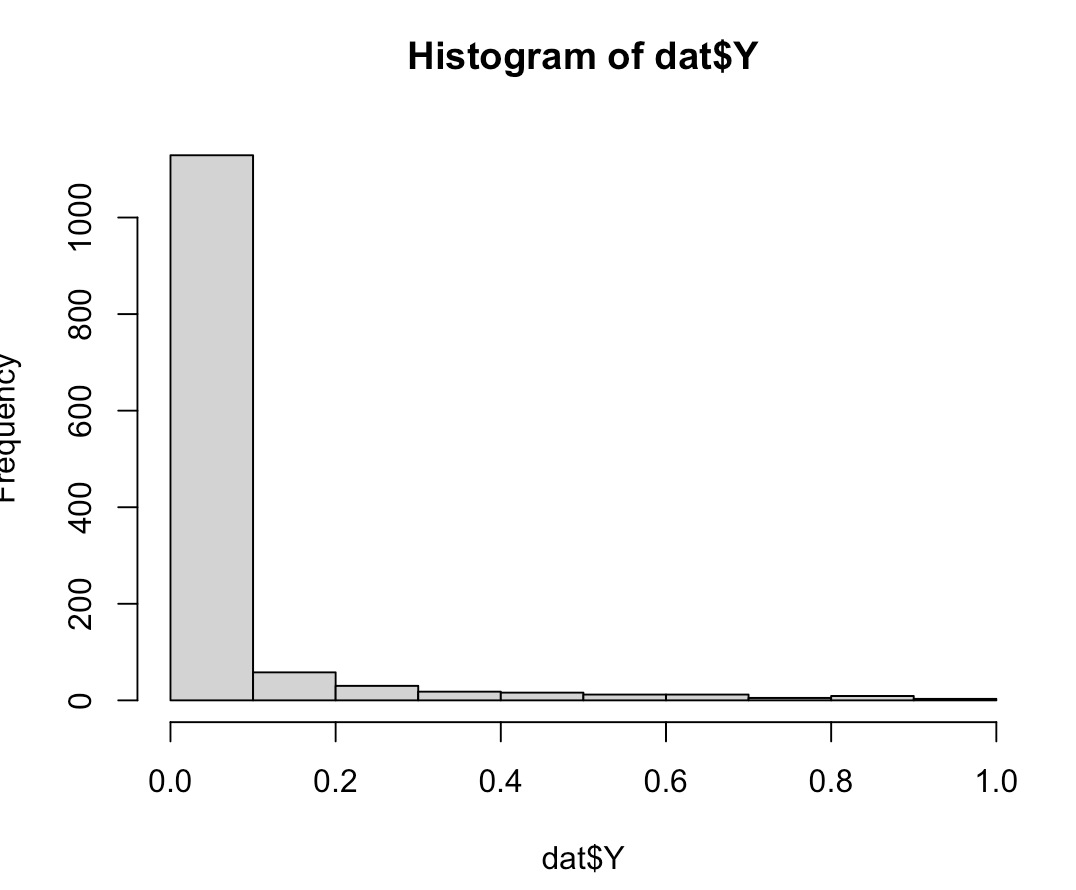
\includegraphics[width=0.45\textwidth]{img/Progress_Report-ce0570ff.png}

Still trying to figure out the best way to define X. As its own, or in big matrix form.


Initializing the $\beta$ column, which is just initializing the intercept, or initializing $\alpha$.

Idea: $\alpha_j = \bar y_j/ \sum_s \bar y_j$
Simpler idea: set everything to zero.

Distance matrix, pass in argument as dist(), then dont need upper.triangular code

Initial iteration
all alpha = 1, alpha0 = p = 19
all diagonals of A are the same (inverse dirichlet variance)

What did we decide about overdispersion?

Is $A$ just the variance? or covariance? It should be covaraince right? No it is variance. Covariance comes from the part of the working correlation matrix, since from variance and correlation we can get covariance.


GEE:

Working COVariance matrix $V_i$

\begin{align*}
  V_i = A_i^{1/2}R_i A_i^{1/2}
\end{align*}
where $R_i$ is the working CORrelation matrix, which should have values between 0 and 1, and should have diagonal entries of 1.


Why is Dirichlet correlation not have diagonal entries of 1? Because covariance is not defined the same if $i = j$. So is it ok we just define the diagonal as 1? I think so.


Back to initialization idea: Using all zeros doesnt work. (maybe for other reasons). Might be the problem since everything is the same? Although the residuals aren't the same after the first iteration. But try to initialize the beta intercept better.


Currently, the code will not finish running. It will not even run to the second iteration. Errors in nls:
Error in nls(y ~ w * r + (1 - w) * exp(-2 * rho * d), data = nls\_data\_frame,  :
  number of iterations exceeded maximum of 50
In addition: Warning message:
In solve(hess, esteq) :
  Exact singularity detected during LU decomposition: U[i,i]=0, i=3.


NLS error comes from the fact that literally everything is NaN, since $\beta$ starts the second loop as all NaN.
If we have more that one iteration in the beta loop beta goes to Nan, likely because we are dividing by zero.

Interestingly, only the first several betas are non-zero.


Maybe also filter samples? Some samples have 0 values for more than 70\% of the ASVs.

Filter samples to only include if less than 40\% of the covariates (ASVs) are non-zero.


FIXED - add phi to the Vi. Seems to give more reasonable beta estimates. Still have error of Warning message:
In solve(hess, esteq) :
  Exact singularity detected during LU decomposition: U[i,i]=0, i=25.

I think this is why the later betas are 0.


With dividing by phi, on the second iteration phi is NaN, since some of the alphas are infinity.




TRY: ignore phylogenetic correlation portion.


Could this be a Matrix package bug? - likely not

Try converting to regular Matrix - still error

Error in solve.default(as.matrix(hess), as.matrix(esteq)) :
  Lapack routine dgesv: system is exactly singular: U[25,25] = 0

IDEA: filter samples so can actually visualize


Check beta updates in loops correctly named

Idea: have the beta loop before nls

TODO: split up update rho, update beta into separate functions

Double check phis

Is it beta + update or beta - update ???????
If this is wrong it could be inflating the values, but this is not where the initial problem comes from.



IDEA: initializing the intercept beta term to $\bar y_i/\sum \bar y_j$. No should be log? Since we are initilizing beta and $\log \alpha_j = X \beta_j$.

Not a good idea, since $\sum \bar y = 1$

Note that there is very little variation among the means of the OTUs across samples!

I think we add the update...
If it is Newton-Rhapson, we subtract, if it is Fisher scoring, we add.
According to GEE paper, it is Fisher scoring, but in the paper, they subtract...


If we divide residuals by square root phi,

\subsection*{Algorithm}

\begin{algorithm}
\caption{An algorithm with caption}\label{alg:cap}
\begin{algorithmic}
\State $y = $ proportions of ASVs
\State $x = $ matrix of covariates
\State $n = $ number of samples
\State $p = $ number of OTUs
\State $q = $ number of covariates + intercept
\State $X = $ kronecker product of covariates
\State Initialize $\beta, \rho, \omega, \alpha, A$
\Loop
  \Loop
  \State $\eta \gets X \beta$
  \State $\alpha \gets e^\eta$
  \State $\mu \gets \alpha/\alpha_0$
  \State $\Delta \gets \frac{1}{\alpha_0^2} ( \alpha_0(\text{diag}(\alpha_i)) - \alpha_i \alpha_i^t ) \otimes x $
  \State $V^{-1} \gets \frac{1}{\phi} A^{-1/2} R^{-1} A^{-1/2}$
  \State Hessian: $H = \Delta V ^{-1} \Delta^t$
  \State Estimating equations $E = \Delta V ^{-1}(Y - \mu)$
  \State update = \texttt{solve(H, E)}
  \State $\beta^+ \gets \eta$ - update
  \EndLoop
  \State $\eta \gets X \beta$
  \State $\alpha \gets e^\eta$
  \State $\mu \gets \alpha/\alpha_0$
  \State $A^{-1/2} \gets \sqrt{\frac{1}{\text{Dirichlet Variance}(\alpha,n,p)}}$ - diagonal matrix
  \State resids:$e \gets A^{1/2}(Y - \mu)$
  \State $\phi \gets \frac{1}{n-(q-1)} e e^t$
  \State Estimate $\omega, \rho$: NLS: \texttt{nls}$(e e^t \sim \omega \text{Cor}_D + (1 - \omega)e^{-2\rho D})$
  Initial values of $\omega = \tfrac{1}{2}, \rho = 1$
  \Comment{If $\rho < 0$, set $\rho = 0$}
  \State $R \gets \omega\text{Cor}_D + (1 - \omega)e^{-2\rho D}$
  \State Solve $R ^{-1} $ by Moore-Penrose Inverse

\EndLoop
\end{algorithmic}
\end{algorithm}

\subsubsection*{Questions}
How is compositionally affected when the majority of taxa contained in original sample are filtered out?

How do we initialize the beta column? Especially the intercept. Because we dont have estimates for the $\alpha$ vector yet, and we dont link $y$s to the $\alpha$s.

How should we initialize the rho vector?

Should the nls omega and rho start at their old values?

\subsubsection*{Email update}
This week I have returned to coding using the zebrafish dataset. I filtered the dataset so it only contains about 20\% zero entries, but I am still running into the same problem I was previously. After the first iteration many of the estimated Dirichlet alpha parameters are infinite. I believe the issue is coming from the step of solving the estimating equations, as the hessian matrix is singular in the first iteration. Can we walk through the code in our meeting Friday to try to figure out where the problem comes from?

\subsubsection*{Meeting agenda}

\hrulefill

\section{October 27}

Having a hard time starting today! Need to write up everything for the presentation on Monday.

Read up more on the evolutionary trait model original paper \cite{Martins1997}
Their version of the correlation assumes that phenotypic evolution (evolution by traits?) is thought to be constrained such that extreme phenotypic values are more likeliy to evolve toward less extreme values. These include evolutionary models that include a stabilizing selection. What does this mean and is it relevant for MB data?

The plan for the rest of the day is to work on the presentation and do work to fill in the gaps.



\section{October 21}


Today I worked mostly on coding the alpha step (correlation) for the evolutionary trait model.

Unfortunately, this assumption forces all correlations to be positive (since the function is $e^{-2\rho d_{ij}}$). This might be too restrictive of an assumption and is not (to my knowledge) biologically supported (and in fact has been biologically rejected theres a paper cited in my masters project)

I focused on coding for the nls part of the updating alpha step. We have the upper triangular (or lower triangular - its arbitrary) part of the distance matrix which has dimensions $p \times p$ where $p$ is the number of OTUs.

Currently no longitudinal component yet.

Had to figure out how to manipulate data.

For the $i$ sample, we find the corresponding $d_{jk}$ where both $j$ and  $k$ are indeces (here) for the OTUs. the response then is $e_{ij}e_{ik}$.

Trying to remember if we decided to make it be nonlinear least squares regression or take the log.

Lets just try the linear version?

But what if $e_{ij}e_{ik}$ is negative? So we cant take the log... They also had this in the AR1 case in the Liang paper.

Additionally, $\rho$ has to be in $(0,\infty)$, ie positive.

Reminder: large $\rho$ means no correlation, small $\rho$ means high correlation.

After trying to take the log of the normalized residuals, it turns out that almost half of the multiplied residuals are negative, making the log infinity. this does not seem like a good basis for running regression as we would have to exclude them all. Is it the absolute value that is calculated??

** Look up how AR1 GEE correlation is usually calculated. - from Liang paper.

Do we use an intercept?

Currently failing with error

Error in nls$(y ~ exp(-2 * x * a)$, data = alpha df, start = c(a = 1)) :
  singular gradient

Also current variance is really small. but comparitively is it/ idk.
Probably the problem is we have negative residuals. and the exponential function is positive. What to do!

Current approach: Take absolute values. This makes the code actually run.

Now we need to invert R.

GeeM code uses R as the block matrix of the entire sample structure. so instead of $p \times p$ it is $np \times np$

Is inverting equivalent??

How do i do this inverting??
Or should I do the old version of systems of equations??

First idea: convert R into Block R and invert using baser functions.

Can I use the fixed format inversion function?

Can I invert the singular R and then make it into a block matrix?

For a block diagonal matrix the inverse is the inverse of the blocks (apparently)

We only need to be fancy when cluster sizes are not the same.


Using solve - R is not invertable! Because of such high values?
Why are values so high!

rho has to be positive- currently negative...

Use the linear model form because that can ensure that rho is positive? jk thats not true

Force intercept at 0? Will this ensure positive rho?
Would significance mean anything here?


Still need to do sandwich estimates.
Look at convergence criteria.


\section{Oct 15 Meeting}

The working correlation assumption using the evolutionary trait model $C(\rho) = e^{-2\rho d_{ij}}$ will assume all positive correlations. This might be too restrictive of an assumption.

What distribution to use for the link and variance functions? Perhaps log-normal, two parts.

New idea: (from Chenyang's GEE clustering paper) Use her ideas of the mean and variance links using Dirichlet multinomial. This will help address compositionally.

How to incorporate her working correlation matrix with mine? Weighted average? New parameter: $\omega \Sigma_1 + (1 - \omega)\Sigma_2$

How to calculate rho? Use linear or non-linear regression to find estimates in each iteration
- REgress (log?) on eijeik ~ e2rhod
But residuals might be negative?

Look up more how Ziegler paper made sure the estimation of $\alpha$ it was not negative?. Because $\alpha$ could be negative but they are using logs.



\section{October 12}

First, consider samples taken on $m$ individuals, indexed $i = 1, \ldots , m$.


Each individual has $p_i$ response OTU measurements taken on it. For simplicity, assume $p_i = p$ for all $i$. OTUs measurements indexed $j = 1, \ldots , p $

$$\mathbf{y}_i = (y_{i1}, \ldots, y_{ij}, \ldots , y_{ip})$$




On each sample there are measured $q$ covariates, such as age, disease status, etc, indexed $k = 1, \ldots, q$
$$\mathbf{X}_i = (\mathbf{x}_{i1}, \ldots, \mathbf{x}_{ik}, \ldots , \mathbf{x}_{iq})^T$$

This matrix $\mathbf{X}_i$ has dimension $p \times q$.

In most cases $\mathbf{x_{ik}} = x_{ik}\boldsymbol{1}_{p \times 1}$, ie values for the $k$th covariate of the $i$th sample is the same for all $p$ OTU observations.


We are trying to code a GEE model for microbiome data. Using \cite{Xiao2018}, based on the evolutionary trait model for correlations between OTUs.


Set up notation for GEEs:

Consider the mean vector $\boldsymbol\mu_i = (E(y_{i1}), \ldots , E(y_{ip}))^t$ and the mean is linked to the covariates through the link

$$g(\boldsymbol\mu_i ) = \mathbf{X}_i \boldsymbol\beta$$

Where $\boldsymbol\beta = (\beta_1 , \ldots , \beta_q)^t$

The variance of the response is a function of the mean

$$\textbf{Var}(\mathbf{y}_{ik}) = \phi a_{ik} = \phi a(\mu_{ik})$$


The generalized estimating equations find the solution $\beta $ to satisfy

$$\sum_{i = 1}^m \bigg(\frac{d \boldsymbol\mu_i}{d \boldsymbol\beta}\bigg)^t \bigg(\mathbf{A}_i^{\frac{1}{2}} \mathbf{R}_i(\alpha) \mathbf{A}_i^{\frac{1}{2}}\bigg)^{-1}(\mathbf{y}_i - \boldsymbol\mu_i) = 0$$


$\mathbf{R}_i(\alpha)$ is known as the \textbf{working correlation matrix}, which is parametrized by the vector $\alpha$.

$\mathbf{A}_i = \phi\text{diag}(a(\mu_{i1}))$


Currently with this formulation, the interpretation for $\beta_k$ is for the expected change in the population average response from changes in the covariate.


\subsection{The GEE algorithm}

The GEE algorithm is an iterative algorithm based off of  alternating between solving the estimating equation for $\beta$ and solving the estimating equation for $\phi$ and $\alpha$.





Trying to get GEE code running. Using ohio dataset from geeM package and data1 from glmmTree package for sanity checks and correctness. Will need to work on filtering the glmmTree dataset more as in current forumulation will not run.

Also going through the geeM code to make modifications to get the basic setup!








\bibliography{cited}
\bibliographystyle{ieeetr}



\end{document}
